\section{Neue Medien - AH}
\textit{Autor: Aurelian Hermand}

Im folgenden Abschnitt werden Hochschultrends im Bereich der „Neuen Medien“ beschrieben. Dabei wird auf das fortschreitende Verlangen nach „Consumerization“, der Wandel zur heterogenen Nutzung der Angebote über verschiedenartige Geräte, der gleichzeitig stattfindende Wunsch zur Zentralisierung der Administration und Infrastruktur und der Imagebildung über das Marketing mit Hilfe unter anderem des Onlineauftritts, der Kommunikation in sozialen Medien und der App-Informationssysteme eingegangen. Die genannten Trends werden nur grob aufgezeigt und in Folgekapiteln aufgegriffen und auf die Hochschule Emden/Leer angewendet.


% ---------------------------------------
\subsection{Infrastruktur und Management}
Die Infrastruktur und das Management an Hochschulen befinden sich seit der Digitalisierung in einem ständigen Wandel. Neue Technologien führen immer wieder zu neuen Begehrlichkeiten, wie z.B. Standardisierung, Zentralisierung oder Prozessorientierung. Im folgenden Abschnitt werden die aktuellen Trends an einigen wichtigen Aspekten betrachtet.


\subsubsection{Netzinfrastruktur, Consumerization und BYOD}
\label{netzinfrastruktur_consumerization_und_byod}
Im Zuge der Consumerization haben sich die Grenzen der Nutzung von privater und beruflicher Software und Geräte aufgelöst. Zum einen bringen Benutzer Software und Hardware mit, die Sie im beruflichen Umfeld verwenden möchten, aber auch umgekehrt, wollen Benutzer beruflich genutzte Software privat nutzen. Eine homogen gestaltete Infrastruktur ist damit hinfällig geworden, in dem Sinne, dass nicht mehr per Vorgabe geregelt wird, eine bestimmte Software- und Hardwarevariante zu verwenden.
Der Trend zum Bring Your Own Device (BYOD) hat veranlasst, dass eine Infrastruktur flexibel 
gestaltet wird. Insbesondere auch die gestiegene Nutzung von Mobilgeräten wie Smartphones 
und Tablets hat dazu geführt, dass Software neuen Vorgaben gerecht werden muss. Gegenüber 
der Steigerung der Produktivität müssen jedoch die Kosten im Auge behalten werden. Im 
Hinblick auf die Implementierung sind dabei Aspekte wie Sicherheit und Infrastruktur zu 
berücksichtigen.\footcite{forrester_research_2012}



Viele Hochschulen in Europa haben sich mittlerweile dem Projekt eduroam (education roaming) angeschlossen. Eduroam ist eine Netzinfrastruktur und ermöglicht die Nutzung von WLAN und LAN an jeder teilnehmenden Hochschule durch vorherige Authentifizierung mit einem Hochschulaccount und einem beliebigen Gerät.
Eduroam als standardisierte Lösung macht die Teilnahme verschiedener Geräte und Standorte im Zuge von BYOD sehr einfach. Geringere Support-Aufwendungen auf der anderen Seite ermöglichen es die Serviceorientierung teilweise abzulösen und durch Prozessorientierung zu ersetzen. Der Aufwand erhöht sich jedoch für die Administratoren durch „die Offenheit der Gerätewahl.“\footcite{wickhill_byod_2013} Der Sicherheitsaspekt spielt daher eine große Rolle. An den Standorten selber kommt es in Folge der Offenheit für die Benutzer wiederum so zur Steigerung der Produktivität und Benutzerzufriedenheit, weil die Arbeitsabläufe flüssiger und effizienter werden.

\subsubsection{Software für Forschung und Lehre}
\label{software_forschung_lehre}
Software- und Service-Anbieter bieten häufig spezielle Angebote für Hochschulangehörige. Eines der bekanntesten ist dabei Dreamspark. Das Netzwerk Dreamspark ermöglicht es Studenten und Bediensteten im Rahmen von Forschung und Lehre kostenlos eine Vielzahl von Microsoft Softwareprodukten zu erhalten und auf Ihren Geräten zu installieren.

Viele Hochschulen, unter anderem die Hochschule Osnabrück, Hochschule Hannover oder auch die Hochschule Emden/Leer ermöglichen die Teilnahme am Dreamspark-Netzwerk.

Neben Dreamspark bieten Hochschulen über Ihre Website Links und Hinweise zu weiteren Angeboten, siehe unter anderem. TH Nürnberg.\footcite{thnuernberg_software_2015} Die zentrale Anlaufstelle für Hochschulangehörige ermöglicht die schnelle Auffindbarkeit und Erkundung in Frage kommender Software, wie zum Beispiel folgender Angebote:

\begin{itemize}
	\item GitHub \footcite{github_edu}
	\item JetBrain \footcite{jetbrains_edu}
	\item Video2Brain \footcite{video2brain_edu}
\end{itemize}


\subsubsection{Identitätsmanagement}
Ein umfassendes Identitätsmanagement setzt eine komplexe Architektur voraus. Die zwei Hauptfunktionen des Identitätsmanagement klassifiziert sich in:

\begin{itemize}
	\item neue Benutzer anlegen
	\item Benutzer entfernen
\end{itemize}

Die Hochschulen gehen die Entwicklung der Zentralisierung vgl. hierzu Kapitel 
\ref{zentralisierung}. Dabei soll die Einrichtung und Löschung der Benutzer-Daten schnell, klar 
und nachvollziehbar hinterlegt werden 
können.\footcite{harnisch_identitat_2008}

Dem Benutzer wird der Zugriff auf die Dienste der Hochschule soweit wie möglich erleichtert, hier wird vor allem auf die Einmalanmeldung (Single-Sign-On) gesetzt. Dem Benutzer werden alle angeschlossenen Dienste der Hochschulen zugänglich gemacht, ohne sich mehrfach Authentifizieren zu müssen. Unter anderem wird dabei auf Shibboleth gesetzt, vgl. Kapitel \ref{shibboleth_sso}.


\subsubsection{E-Mail}
Ein integraler Bestandteil an Hochschulen ist die E-Mail Infrastruktur. Der Trend geht zu einem zentral-administrierbaren System. Im Sinne des Consumerization wird die Nutzung des E-Mail Services offen gestaltet für alle vorstellbaren Endgeräte und Programme. Die zentralen Systeme gewähren die heterogene Nutzung über Desktop, Mobilgeräte und Webmailer. \footcite{hszwickau_zahlen_2015}


\subsubsection{E-Learning Plattform}
\label{subsubsection_e_learning_plattformen}
Das elektronische Lernen setzt auf den Einsatz digitaler Medien. Das Blended Learning vereint das Präsenzstudium mit dem E-Learning und hat dabei drei substantiell wichtige Lerndomänen

\begin{itemize}
	\item das lernen online durch Kommunikation
	\item distanziert ohne Interaktion
	\item und in der Präsenz.
\end{itemize}

Auch im Präsenzstudium wird zunehmend nicht nur auf offline Medien Skripte oder Bibliothek gesetzt, sondern zusätzlich auf Aufzeichnungen, Videochats, online Einsendeabgaben und Foren.

An Hochschulen wird zum gr\"oßten Teil auf eine der zwei größeren Plattformen gesetzt.\footcite{oevel_lange_2008}

\begin{itemize}
	\item Moodle www.moodle.com
	\item ILIAS www.ilias.de
\end{itemize}

Die Plattformen waren ursprünglich für das Onlinestudium gedacht, ziehen jedoch mehr und mehr in das Präsenzstudium ein. Dabei wird das Potential der Plattform noch selten ausgereizt und ist nicht verpflichtend. Sie erweitern das Präsenzstudium aber um zusätzliche Möglichkeiten.
Neben dem Platzhirsch wie Moodle vgl. Kapitel \ref{paragraph_moodle} werden noch weitere Systeme wie Lon-Capa und StudIP eingesetzt.

Die Plattformen ermöglichen es, dass Skripte zur Verfügung gestellt und kontinuierlich weiterentwickelt werden können. Dabei ist auch die Kooperation mehrerer Autoren und Outsourcing möglich, vgl. auch Kapitel \ref{outsourcing}. Um diese Skripte entsteht dann ein Ökosystem aus Übungsaufgaben, Videos und Forenbeiträgen.



% ---------------------------------------
\subsection{Dokumentenverwaltung}
\label{dokumentenverwaltungssysteme}
Im Abschnitt Dokumentenverwaltung wird auf die an Hochschulen eingesetzten Software-Trends und auf das Druckzentrum der Uni Münster eingegangen.


\subsubsection{Wiki}
Das Wiki ist ein Dienst zur Erfassung ungeordneter, miteinander verknüpfbarer Texte. Sie sind sehr flexibel einsetzbar und werden daher von sehr vielen Hochschulen eingesetzt. Es lassen sich schnell Informationen versionsbasiert gemeinsam zusammentragen und verwalten.\footcite[Vgl.][65]{schmidtjh_2013}

Wikis stellen oft die erste Basis für Informationsverwaltungen, aus denen konzentriertere Informationssysteme entstehen können in Form von Websites oder auch FAQs, Anleitungen und vieles mehr.


\subsubsection{Clouds und Big Data}
Clouds ermöglichen den einfachen Datenaustausch großer Dateien mit verschiedenen Zugriffsrechten. Eingeteilt werden können die Clouds in

\begin{itemize}
	\item öffentliche Clouds
	\item private Clouds
	\item hybride Clouds
	\item community Clouds
\end{itemize}

Die private Cloud ist im Gegensatz zur öffentlichen Cloud ein geschlossenes System für ein meist festgelegten Nutzerkreis oder einer Einzelperson und wird hauptsächlich aus Gründen des Datenschutz und Sicherheit eingesetzt.
Die hybride Cloud ist eine Mischform aus zwei einzelnen Cloud-Formen die miteinander verbunden werden, dabei werden die Eigenschaften der verknüpften Clouds erhalten. Dies ermöglicht einen flexibleren Einsatz.
Die Community Cloud stellt einem definierten Nutzerkreis von mehreren Standorten Zugriff auf die Cloud zur Verfügung. Hierbei wird gemeinsam oder von einem Anbieter die Cloud verwaltet.\footcite[Vgl.][3]{nistpub_2011}
Ein Beispiel dieser Community Cloud wird an den Hochschulen in NRW im Verbund eingesetzt. Dahinter steckt die Software ownCloud und wird „Sciebo die CampusCloud“ genannt.

Die Hochschule Emden/Leer führt derzeit mit Hilfe des Shibboleth-Dienstes eine Cloud namens „Gigamove“ zum Austausch großer Datenmengen ein. Gigamove wird von der RWTH Aachen zur Verfügung gestellt\footnote{\url{https://gigamove.rz.rwth-aachen.de}}. Weitere Details werden im Kapitel \ref{gigamove_rwth_aachen} behandelt.

„Big Data“ wird eingesetzt, um die ständig wachsenden Datenmengen verarbeiten zu können. Allgemein wird der Begriff „Big Data“ verwendet, wenn eine Datenmenge mit herkömmlichen Rechnern nicht verarbeitet werden kann. Außerdem liegen die Daten in vielen strukturierten und unstrukturierten Formaten vor. Die Entwicklung zielgerichteter Software zur Beantwortung von Forschungsfragen ist dabei die wichtigste Aufgabe. Sie kann Hochschulen bei der Lösung oder Visualisierung von größeren Problemstellungen helfen.\footcite[Vgl.][65]{keller_klein_tuschl_2015}


\subsubsection{Versionsverwaltung}
Die Versionsverwaltung dient allgemein zur Dokumentenerstellung, -bearbeitung und -verwaltung. Dabei ist 
es jederzeit möglich auf einen vorhergehenden Stand zurückzusetzen oder Änderungen nachvollziehen zu 
können, damit auch ein kollaboratives Arbeiten an einem Dokument möglich ist. Die Uni Kassel setzt auf die 
Dokumentenmanagement Software Alfresco. Alfresco ist ein bequemes und unkompliziertes System mit dem 
verschiedene Dokumente und Dateien zentral verwaltet werden können. Die Software bietet Features wie 
Benutzerverwaltung, Integration in Moodle, Workflows zur Dokumentenüberprüfung, Aufgabenverteilung, 
Zusammenfassung oder Versionierung von Office- oder PDF-Dokumenten. Außerdem existieren Apps für 
mobile Endgeräte.\footcite{unikassel_dms_2015}


\subsubsection{Zentrales Druckzentrum}
Das ZIV (Zentrum für Informationsverarbeitung) der Uni Münster zentralisiert unter anderem die Rechnerräume und unterhält ein Druckzentrum. Das Druckzentrum bietet den Service Ausdrucke von überall aus zu veranlassen, sei es über stationär mit einem Desktop-PC oder unterwegs mit einem mobilen Endgerät. Die Ausdrucke werden serviceorientiert in einem zugeordneten Postfach einsortiert mit einem farbigen Deckblatt und können von dort zu einem späteren Zeitpunkt aus dem Fach genommen werden können.
\footcite{wwu_printnpay_2014}



% ---------------------------------------
\subsection{Außendarstellung und Marketing Instrumente}
\label{aussendarstellung_und_marketing_instrumente}
Das Marketing und die Präsentation der Hochschule erfolgt breit gefächert und geht im Idealfall fließend ineinander über. Die Trends erfolgen oft in Organisatorischen Maßnahmen\footcite[Vgl.][4f.]{bode_2008}. D.h. es wird am Ausbau und Vereinheitlichung gearbeitet, im Sinne von Corporate Identity bzw. Corporate Design der Webdienste, E-Learning Plattform, zentrale Datenspeicher, Verwaltungs EDV und sonstigen Angeboten.

\subsubsection{Website}
Die Website ist ein integraler Bestandteil der Hochschulen. Alle relevanten Informationen werden für die Website aufbereitet und den Benutzern intern und extern zugänglich gemacht. Der technische Fortschritt, verlangt zudem Beachtung neuer Designkriterien, um die Sichtbarkeit im Internet zu gewährleisten.

\paragraph{Responsive Website}\mbox{}\\\\
Responsivität im Webdesign heißt, das im Sinne des BYOD, der Zugriff auf die Hochschul-Website komfortabel und geräteunabhängig gestaltet ist. Die Fachhochschulen Köln und Münster sind dem Trend gefolgt, jedoch ohne auf einen etablierten Marktstandard zu setzen.

Auf dem Markt gibt zwei sehr verbreitete Frameworks, die meist aus Sammlungen von Modulen, Grids und Best-Practices bestehen, wie dem Prinzip des Mobile First. Mobile First bedeutet, dass aus Gründen des meist kleineren Bildschirms der Fokus auf den Inhalt liegt. Hiermit wird auch gleichzeitig das Prinzip des „Content First“ bzw. „User First“ umgesetzt. Sowohl Bootstrap\footnote{\url{http://getbootstrap.com/}} von Twitter als auch Foundation von Zurb\footnote{\url{http://foundation.zurb.com/}} gelten als ausgereifte Frameworks. Die Verständigung auf ein ausgereiftes System, kann eine kostenintensive und proprietäre Selbstentwicklung verhindern. Twitter Bootstrap wird beispielsweise unter anderem von der Hochschule Coburg und der TU München eingesetzt.

Die responsive Umsetzung mit Mobile First erhöht deutlich die Gebrauchstauglichkeit (engl. Usability), weil die Website auf dem mobilen Endgerät nicht gezoomt werden muss und so ausgeliefert wird, wie die Designer und Konzepter es konzipiert haben.

Die neueste Entwicklung im Bereich der responsiven Umsetzung erfolgte durch die Änderung des Suchalgorithmus von Google im April 2015. Die Änderung betrifft die Bewertung mobil optimierter Websites in den Suchergebnissen, die fortan bevorzugt gelistet werden, sofern über ein mobiles Endgerät gesucht wird.\footnote{\url{http://www.heise.de/newsticker/meldung/Google-Mehr-mobile-als-Desktop-Suchabfragen-2635987.html}}


\paragraph{Sichtbarkeit und SEM}\mbox{}\\\\ 
Das Suchmaschinen-Marketing wird zusammengefasst unter dem Kürzel SEM (Search-Engine-Marketing). SEM umfasst die Konzepte SEO (Search-Engine-Optimization) und das SEA (Search-Engine-Advertising).\footcite[Vgl.][83]{kr_ru_wiba_2015}

Die Suchmaschinen-Werbung bzw. SEA wird genutzt, um gezielt bestimmte Suchbegriffe gegen Bezahlung auf der ersten Seite der Suchmaschinen als Werbung einzublenden.

Unter SEO versteht man die allgemeinen Suchmaschinen-Optimierungs-Maßnahmen, um im organischen Ranking weit vorne zu landen.

Auswirkungen des SEM können unter anderem mit Hilfe des Sichtbarkeitsindex ermittelt werden. Der Sichtbarkeitsindex dient als Indikator für die Sichtbarkeit einer Website im Google Ranking. Dabei errechnet sich der Index aus:

\begin{itemize}
	\item dem Ranking der thematisch überwachten Keywords
	\item dem zu erwartenden Traffic aus der Positionierung und
	\item dem zu erwartenden Traffic aus dem Keyword.
\end{itemize}

Der Sichtbarkeitsindex wird als ein weiterer Messwert herangezogen für den Erfolg von SEO-Maßnahmen, neben unter anderem Zugriffszahlen und Verweildauer der Besucher.\footnote{\url{https://de.onpage.org/wiki/Sichtbarkeitsindex}}

Die www.hs-emden-leer.de erreicht laut SISTRIX im Mai 2015 einen Sichtbarkeitsindex von 0,31. Im Vergleich dazu erreicht www.hs-coburg.de 0,62 und www.jade-hs.de 0,69.\footnote{\url{http://www.sichtbarkeitsindex.de/}} Je höher der Index ist, desto sichtbarer ist die einzelne Hochschule aufgestellt. Hochschulen mit einem niedrigeren Index hätten demnach noch Potential und können die Maßnahmen der Wettbewerber als Inspiration nutzen.

\paragraph{Inhaltsaufbereitung}\mbox{}\\\\
Der wichtigste Teil einer Website ist der Inhalt selber, der Fokus hier liegt auf der Vollständigkeit und einer verständlichen Sprache. Die Texte werden oft in verschiedenen Formaten präsentiert, d.h. zum Beispiel in sozialen Medien, PDFs, Drucklayouts, XML-Sitemaps und RSS ausgegeben.

RSS (Rich Site Summary) ist dabei ein XML-Format zur Übertragung vorallem von News, Terminen und sonstigen Informationen. Der Benutzer kann dieses Format mit eigenen Programmen abonnieren und bleibt so auf dem laufenden.




\subsubsection{Social Media}
„Social-Media-Marketing (SMM) ist eine Form des Online-Marketings, die Branding- und Vertriebsziele durch ein Engagement in einem oder in verschiedenen sogenannten Social- Media-Angeboten erreichen will.“\footcite[Vgl.][31]{lammenett_2014}

Newsletter Kampagnen sind ein trotz vieler neuer Medien weiterhin ein wichtiger Baustein im Online-Marketing-Mix. Es gibt einen klaren Trend in Richtung hin zu Mobilgeräten. Die Öffnungsraten auf mobilen Endgeräten sind seit 2010 bis 2013 um 300 Prozent angestiegen und übertreffen mittlerweile auch die Öffnungsraten der gewöhnlichen Desktop-Geräte. Betreiber des E-Mail-Marketing setzen umso mehr auf die Optimierung der Kampagnen auf mobile Endgeräte \footnote{\url{Praxiswissen Online-Marketing - S.35}}. Um den Wiedererkennungseffekt zu fördern und die eigene Marke zu etablieren, sollte beim Marketing auf das Corporate Design gesetzt werden.

Dem Social-Media-Marketing stehen unzählige weitere Vertriebskanäle zur Verfügung, wie Facebook, Twitter oder YouTube. Wichtig ist dabei vorher ein Leitbild zu entwickeln und beizubehalten. \footnote{\url{http://www.hs-merseburg.de/fileadmin/_migrated/content_uploads/090219_Marketingkonzept_Final.pdf S.8}}

\begin{figure}[h!]
	\centering
	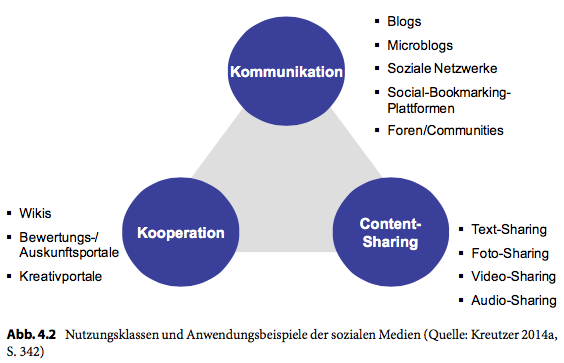
\includegraphics[width=10cm]{kapitel/gruppe1_2/bilder/nutzungsklassen}
	\caption{Nutzungsklassen und Anwendungsbeispiele sozialen Medien (Quelle: B2B Online-Marketing und Social Media, S. 152)}
	\label{fig_nutzungsklassen}
\end{figure}

Die Soziale Medien können auf vielfältige Weise genutzt werden. Die Nutzungsklassen, siehe Abbildung \ref{fig_nutzungsklassen} der sozialen Medien können in drei Bereiche aufgeteilt werden:


\begin{itemize}
	\item Kommunikation: Blogs, Microblogs, Soziale Netzwerke, Social-Bookmarking-Plattformen, Foren/Communities
	\item Content-Sharing: Text, Foto, Video, Audio
	\item Kooperation: Wikis, Bewertungs-/Auskunftsprotale, Kreativportale
\end{itemize}

Die Nutzungsklasse \ref{fig_nutzungsklassen} „Kommunikation“ zielt darauf ab, aufbereitete Informationen über private und professionelle Netzwerke bereitzustellen und zu diskutieren.
Ähnlich der Nutzungsklasse „Kommunikation“ zielt auch das „Content-Sharing“ darauf Inhalte zu teilen über spezifische Media-Sharing Plattformen.
Bei der Nutzungsklasse „Kooperation“ steht vor allem die gemeinsame Aufbereitung von Informationen im Mittelpunkt.

Social Media spielt für die Rekrutierung neuer und Erreichbarkeit bestehender HS-Interessierter eine wichtige Rolle. Hierüber können Angebote, Stellenausschreibungen geschehen. Diese können dann verlinkt und geteilt werden. 

Eine Integration in die Website sollte Datenschutzrechtlich vorgenommen werden, bspw. mit der 2-KLick-Technik.




\subsubsection{App als Informationssystem}
\label{android_app_als_is}
Der Trend an Hochschulen geht zu Informationssystemen in Apps bzw. Webapps. Ein allgemeiner Trend dabei ist das Prinzip die Apps so zu entwerfen, dass sie sowohl offline als auch online funktionieren. Dieses Prinzip nennt sich „Offline First“.

\begin{figure}[h!]
	\centering
	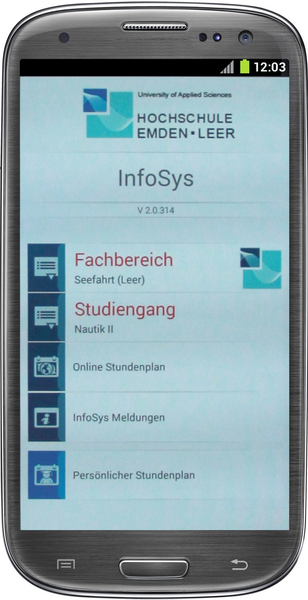
\includegraphics[width=10cm]{kapitel/gruppe1_2/bilder/hsel-androidapp}
	\caption{Android App der HS Emden / Leer}
	\label{fig_hselandroidapp}
\end{figure}

Die Hochschule Emden/Leer ist dem Trend gefolgt und hat Anfang 2014 eine Android App im Rahmen einer Projektarbeit vorgestellt, siehe Abbildung \ref{fig_hselandroidapp}. Das Prinzip „Offline First“ wurde dabei berücksichtigt. Ein Hauptaugenmerk wurde auf die Integration von InfoSys und die individuellen Einstellungsmöglichkeiten der Studenten gelegt, um unter anderem den Stundenplan anzupassen.\footnote{\url{http://www.hs-emden-leer.de/aktuelles-termine/news/article/immer-up-to-date-dank-neuem-smartphone-app.html}}

Da die Entwicklung im Rahmen einer Projektarbeit vonstatten ging, wird es sehr wahrscheinlich bei dieser einen Version und dem einzigen Gerätetyp bleiben.

\begin{figure}[h!]
	\centering
	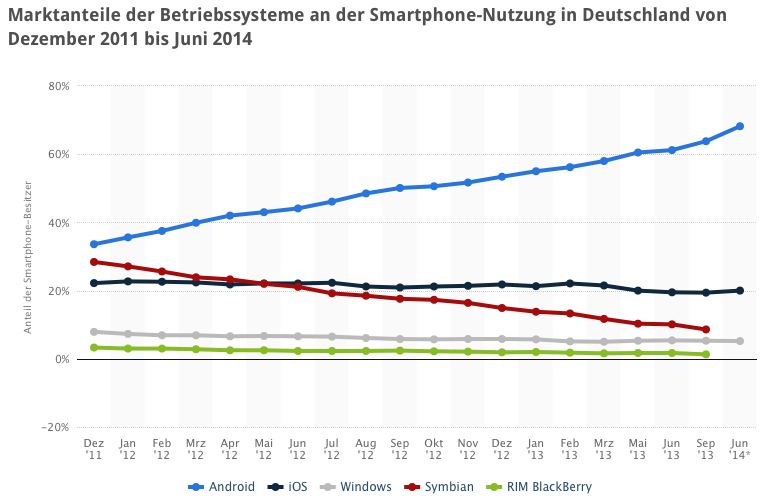
\includegraphics[width=10cm]{kapitel/gruppe1_2/bilder/marktanteile}
	\caption{Marktanteile der Betriebssysteme an der Smartphone-Nutzung in Deutschland von 2011 bis 2014}\protect \footnotemark
	\label{fig_marktanteile}
\end{figure}\footnotetext{\cite{statista_markanteile_smartphone_2015}}

An Hand der Marktanteile\ref{fig_marktanteile} werden u.a. 20 Prozent iOS Nutzer nicht berücksichtigt und ist daher nicht im Sinne von BYOD, da eine Beschränkung vorliegt. Der Grund dafür liegt an den Unterschieden der Betriebssysteme. Für jedes System muss prinzipiell eine eigene App entwickelt werden. Ein kostengünstiger Lösungsansatz ist der Einsatz ausgereifter Javascript Webapp-Frameworks, wie beispielsweise Sencha Touch\footnote{\url{http://www.sencha.com/products/touch/}} und AngularJS\footnote{\url{https://angularjs.org/}}. Die Apps lassen sich so mit jedem Gerät zunächst einmal als Website auf dem Mobilgerät öffnen und mit Hilfe von Cordova/Phonegap\footnote{\url{http://cordova.apache.org/}} ist es weiterhin möglich diese Webapps in den wichtigsten App Stores auszuliefern. Einige Hochschulen bieten solche flexible Webapps an, so zum Beispiel die Hochschule Zwickau.\footnote{\url{https://mobile.fh-zwickau.de/}}

Nicht nur Flexibilität im Bezug auf Geräteunabhängigkeit wird geschaffen, auch Hürden der Weiterentwicklung werden verringert, weil auf ausgereifte Software gesetzt wird.

Im folgenden werden ein paar Funktionalitäten einiger Hochschul-Apps aufgezeigt.

\paragraph{InfoSys und News}\mbox{}\\\\
An einigen Hochschulen, wie der Hochschule Heidelberg werden unter anderem Hochschulinformationen und aktuelle Nachrichten direkt über eine App ausgeliefert. Die Integration des InfoSys (vgl. Kapitel \ref{fachbereiche_infosys}) und der aktuellen Nachrichten der Hochschule sind vorhanden, jedoch existieren diese Informationen nur für Android Benutzer.

\paragraph{HIS (Notenzugriff, Stundenpläne)}\mbox{}\\\\
Die HAW Hamburg und auch die Hochschule Heidelberg ermöglicht in der App den Zugriff auf Stundenpläne, Raumpläne, Prüfungen und Noten.\footnote{\url{https://itunes.apple.com/de/app/haw-hamburg/id670347114?mt=8}} Die Hochschule Emden/Leer hat in der Android-App nur den Zugriff auf die Stundenpläne. Die Hochschulen versuchen in Ihren Apps möglichst alle Informationen auszuliefern. Problematisch werden oftmals die Schnittstellen sein. 

\paragraph{Mensa}\mbox{}\\\\ 
Hochschulen haben nicht selten, entweder eine spezielle App nur für die Speisepläne oder sie integrieren die Speisepläne direkt in die eigene Hochschul-App. Die Hochschule Emden/Leer hat derzeit keine spezielle Speiseplan-App. Das Studentenwerk Oldenburg bietet jedoch eine App\footnote{\url{http://itunes.com/apps/MensaplanOL}} für iOS an, bei der auch die Hochschule Emden/Leer integriert ist. Derzeit wird laut dem Studentenwerk Oldenburg an einer neuen Webapp für die Speisepläne gearbeitet. Ein Beispiel für ein gelungenes Projekt bietet die Hochschule Osnabrück, sowohl für iOS und Android.\footnote{\url{http://www.studentenfutter-os.de/}}

\paragraph{Gelände-Wegweiser IPS}\mbox{}\\\\
Ein Indoor Positioning System mit beispielsweise Beacons bzw. Triangulation ermöglicht die Standortbestimmung innerhalb von Gebäuden. Das Auffinden eines Raums in neuen bzw. unbekannten Gebäuden mit Hilfe dieser Technologie und einem mobilen Endgerät, ist damit problemlos möglich. Die Uni Hohenheim bietet dieses Feature als „Hörsaal-Finder mit Live-Navigation“\footnote{\url{https://itunes.apple.com/de/app/universitat-hohenheim-die/id490603166?mt=8}} an, siehe Abbildung \ref{fig_livenavi}.

\begin{figure}[h!]
	\centering
	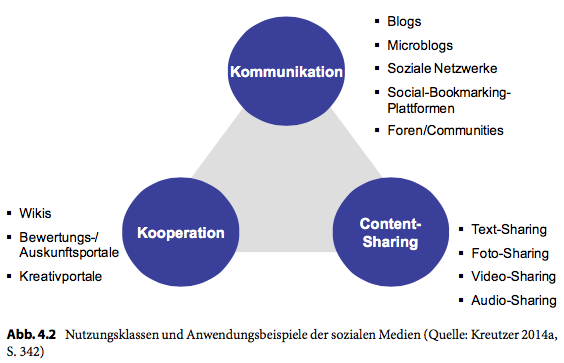
\includegraphics[width=10cm]{kapitel/gruppe1_2/bilder/nutzungsklassen}
	\caption{Hörsaal-Finder der Uni Hohenheim}
	\label{fig_livenavi}
\end{figure}

